\section{Tree caching with dependencies} \label{tree_caching_algo} The problem
that we consider (called \textit{tree caching problem}), introduces an extension
of standard caching problem with bypassing, which was described in section 2.
The main difference between them is, that requested items have some
inter-dependencies. Specifically, their universe forms rooted tree $T$ and the
requested items are placed in its nodes.  Whenever $v \in T$ is fetched, all of
its descendants (denoted $T(v)$), that are not in the cache, have to be fetched
as well. We say, that the cache with property described above, is
\textit{bottom-contiguous}.

Moreover, we consider two types of requests: \textit{negative} and
\textit{positive}. If incoming request is positive we pay 1, if and only if it
is not present in the cache (so like in previously considered settings). On the
other hand, we have to pay for negative requests, if and only if the item is
present in the cache at that time (so in the opposite situation to the positive
requests). After serving the request, we can reorganize the cache, paying
$\alpha \geq 1$ for every element, which is evicted or fetched. 

The goal is to find an online algorithm, that solves this problem and minimizes
the obtained cost. We present a deterministic algorithm \textbf{TRC}, which we
prove is $O(h(T) \times R)$-competitive, where $h(T)$ is height of input tree
and $R = k_{\mathrm{ONL}}/(k_{\mathrm{ONL}} - k_{\mathrm{OPT}} +1)$ with
$k_{\mathrm{ONL}}$ and $k_{\mathrm{OPT}}$ denoting the size of the online and
the optimal offline algorithm's cache respectively.

\subsection{Model} \begin{wrapfigure}{r}{0.6\textwidth}
\begin{postscript}

\psscalebox{0.6 0.6} % Change this value to rescale the drawing.
{
\begin{pspicture}(0,-4.0099998)(12.562361,4.0099998)
\definecolor{colour0}{rgb}{0.78431374,0.78431374,0.78431374}
\psbezier[linecolor=black, linewidth=0.04, 
fillstyle=solid,fillcolor=colour0](4.8323607,3.9899998)(3.8323605,
3.9899998)(0.046042196,0.2078214)(0.8323605,-0.41000015)(1.6186789,
-1.0278217)(9.759687,-1.1499403)(10.432361,-0.41000015)(11.105033,
0.32993993)(5.8323607,3.9899998)(4.8323607,3.9899998)
\pscircle[linecolor=black, linewidth=0.04, fillstyle=solid,fillcolor=black, 
dimen=outer](4.8323607,2.79){0.4}
\pscircle[linecolor=black, linewidth=0.04, fillstyle=solid,fillcolor=black, 
dimen=outer](3.2323606,1.9899999){0.4}
\pscircle[linecolor=black, linewidth=0.04, fillstyle=solid,fillcolor=black, 
dimen=outer](4.8323607,1.1899998){0.4}
\pscircle[linecolor=black, linewidth=0.04, fillstyle=solid,fillcolor=black, 
dimen=outer](6.4323606,1.9899999){0.4}
\pscircle[linecolor=black, linewidth=0.04, fillstyle=solid,fillcolor=black, 
dimen=outer](8.03236,1.1899998){0.4}
\pscircle[linecolor=black, linewidth=0.04, fillstyle=solid,fillcolor=black, 
dimen=outer](7.6323605,-0.41000015){0.4}
\pscircle[linecolor=black, linewidth=0.04, fillstyle=solid,fillcolor=black, 
dimen=outer](9.232361,-0.0100001525){0.4}
\psline[linecolor=black, linewidth=0.04](4.8323607,2.79)(3.2323606,1.9899999)
\psline[linecolor=black, linewidth=0.04](4.8323607,2.79)(4.8323607,1.1899998)
\psline[linecolor=black, 
linewidth=0.04](4.8323607,2.79)(6.4323606,1.9899999)(6.4323606,1.9899999)
\psline[linecolor=black, 
linewidth=0.04](6.4323606,1.9899999)(8.03236,1.1899998)(7.6323605,
-0.41000015)(8.03236,1.1899998)(9.232361,-0.0100001525)(9.232361,-0.41000015)
\psline[linecolor=black, 
linewidth=0.04](3.2323606,1.9899999)(3.2323606,1.9899999)
\psline[linecolor=black, 
linewidth=0.04](4.8323607,2.79)(4.8323607,2.79)(4.8323607,2.79)
\pstriangle[linecolor=black, linewidth=0.06, 
dimen=outer](1.2323605,-3.6100001)(2.4,2.8)
\pstriangle[linecolor=black, linewidth=0.06, 
dimen=outer](4.8323607,-3.6100001)(2.4,2.8)
\psline[linecolor=black, 
linewidth=0.04](4.8323607,0.78999984)(4.8323607,-0.8100002)(4.8323607,
-0.8100002)
\pstriangle[linecolor=black, linewidth=0.06, 
dimen=outer](9.232361,-3.6100001)(2.4,2.8)
\psline[linecolor=black, 
linewidth=0.04](2.8323605,-0.0100001525)(2.8323605,-0.0100001525)(2.8323605,
-0.0100001525)(2.8323605,-0.0100001525)
\rput(11.63236,1.9899999){Tree cap}
\rput(9.232361,-0.0100001525){\textcolor{white}{\textbf{r}}}
\pspolygon[linecolor=black, linewidth=0.04, fillstyle=vlines, 
hatchwidth=0.028222222, hatchangle=0.0, 
hatchsep=0.1411111](2.4323606,-3.6100001)(1.6323606,-2.41)(1.2323605,
-2.8100002)(0.8323605,-2.0100002)(0.032360535,-3.6100001)(0.032360535,
-3.6100001)
\pspolygon[linecolor=black, linewidth=0.04, fillstyle=vlines, 
hatchwidth=0.028222222, hatchangle=0.0, 
hatchsep=0.1411111](4.4323606,-3.6100001)(4.8323607,-2.41)(6.0323606,
-3.6100001)(6.0323606,-3.6100001)
\psframe[linecolor=black, linewidth=0.04, fillstyle=vlines, 
hatchwidth=0.028222222, hatchangle=0.0, hatchsep=0.1411111, 
dimen=outer](10.432361,3.1899998)(9.63236,2.3899999)
\rput(11.63236,2.79){Valid cache }
\psline[linecolor=black, 
linewidth=0.04](9.232361,-1.6100001)(9.232361,-1.6100001)(9.232361,
-1.6100001)(9.232361,-1.6100001)
\psline[linecolor=black, 
linewidth=0.04](9.232361,-0.0100001525)(9.232361,-0.8100002)(9.232361,
-0.8100002)
\pstriangle[linecolor=black, linewidth=0.06, linestyle=dotted, 
dotsep=0.10583334cm, fillstyle=vlines, hatchwidth=0.02, hatchangle=0.0, 
hatchsep=0.2212, dimen=outer](9.232361,-4.01)(4.0,5.2)
\psline[linecolor=black, 
linewidth=0.04](3.2323606,1.9899999)(1.2323605,-0.8100002)(1.2323605,-0.8100002)
\psline[linecolor=black, 
linewidth=0.04](3.2323606,1.1899998)(3.2323606,1.1899998)
\psline[linecolor=black, 
linewidth=0.04](4.8323607,3.59)(4.8323607,3.59)(4.8323607,3.59)(4.8323607,3.59)
\psframe[linecolor=black, linewidth=0.04, fillstyle=solid,fillcolor=colour0, 
dimen=outer](10.432361,2.3899999)(9.63236,1.5899998)
\psframe[linecolor=black, linewidth=0.064, linestyle=dotted, 
dotsep=0.10583334cm, fillstyle=solid, 
dimen=outer](10.432361,3.9899998)(9.63236,3.1899998)
\rput(11.63236,3.59){T(r)}
\end{pspicture}
}

\end{postscript}
\caption{Visualization of definitions.}
\label{fig:TreeCacheDefinitions}
\end{wrapfigure} For ease of the algorithm description
and readability of presented proofs, we introduce bunch of useful definitions.
First of all, by $T(r)$ we indicate the subtree of $T$ rooted in $r$ and by
$h(T)$ the height of the tree $T$.  \textit{Tree cap} is a tree $T_c \subseteq
T$, such that root $r$ of $T$ belongs to $T_c$ and the fact, that $v \in T_c$
implies, that all of the nodes, that lie on the path from $v$ to $r$, belong to
$T_c$.  We say, that set $C \subseteq T$ is \textit{bottom contiguous}, if $v
\in C$ implies $T(v) \subseteq C$ and we call $C$ a \textit{valid cache state}.
Notice that this definition does not depend on the cache size, so $C$ can be
valid cache state and at the same time may not fit into the cache size.

The \textbf{TRC} algorithm, after each request, can change the state of its
cache. The only changes that are possible leave the cache in a valid state.
Depending on the character of change (eviction vs. fetch), we can apply either a
\textit{valid negative changeset} or a \textit{valid positive changeset} on the
cache $C$. The valid positive changeset $X$ (you may think of it as a set that
can be fetched legally) is a set for which $X \cap C = \varnothing$ and $C \cup
X$ is a valid cache state, the negative one (related to eviction) is a set $X
\subseteq C$ such that $C \setminus X$ is a valid cache state.

We process the input one request by one and assume, that each request $\sigma_t$
comes in the time interval $(t-1, t)$. The next request comes in the time
interval $(t, t + 1)$ and so on and so forth. At time $t$ algorithm changes its
cache state from $C_{t}$ to $C_{t+1}$. The cache state is well defined for round
$t$ (which contains time interval $(t-1, t)$), because as we can see, the cache
may only change between rounds.

Some of the definitions, which were introduced above, are presented in the
Figure ~\ref{fig:TreeCacheDefinitions}.

\section{Motivation}

\subsection{Algorithm TRC}

Before defining the \textbf{TRC} algorithm, we bind to each node $v \in T$ a
$bank_{t}(v)$ value. At the beginning of the algorithm, for each $v \in T$ we
have $bank_{0}(v) = 0$. If node $v$ gets a negative or a positive request at
time $t$, whose processing cost us 1, we increase $bank_{t}(v)$ value by 1 (so
$bank_{t}(v) = bank_{t-1}(v) + 1$), leaving the value assigned to any other node
unchanged (so for $v' \neq v bank_{t-1}(v') = bank_{t}(v')$). When we change the
state of node $v$ (either by evicting or fetching it into the cache) we 'clear'
its bank value (change it to $0$). For set of nodes $V \subseteq T$, we denote
sum $\sum_{v \in V} bank_{t}(v)$ by $bank_{t}(V)$.

The \textbf{TRC} proceeds in phases. First phase starts at time 0 and at the
start of each phase the \textbf{TRC}'s cache is empty.  \begin{algorithm}
\caption{\textbf{TRC}} \label{alg:TRC} \begin{algorithmic}[1] \ForAll{$t \in \{1
\ldots |\sigma|\}$} \State Serve request $\sigma_t$.  \State Update $bank_t(v)$
values for $v \in T$.  \If{exists valid changeset $X$ such that: \begin{itemize}
\item $bank_t(X) \geq |X| \times \alpha$ (saturation), \item $bank_t(Y) < |Y|
\times \alpha$ for any valid changeset $Y \varsupsetneq X$ (maximality):
\end{itemize}} \State Apply $X$.  \If {the cache size $k_{\mathrm{ONL}}$ is
exceeded}: \State Empty the cache.  \State Reset all $bank_t$ values to 0.
\State Start new phase.  \EndIf \EndIf \EndFor \end{algorithmic} \end{algorithm}

In line 6 of the algorithm above we do not literally exceed the cache. Instead,
we do not apply last valid changeset, but we empty the cache and start new
phase. From now on this not performed fetch will be called \textit{an artificial
fetch}.  Each phase ends whenever applying valid changeset $X$ would lead to the
cache overload. Only the last phase is treated differently: it can be
\textit{unfinished} (do not end with exceeding the cache size). 

In the body of the algorithm \ref{alg:TRC} there are two properties defined:
\textit{saturation} and \textit{maximality}. The first one is used to express,
that (saturated) changeset is ready to be applied. The latter one ensures, that
applied changeset is the maximal possible at the moment, where the changesets
are ordered by the inclusion order. From the formulation of \textbf{TRC}, every
changeset applied by the algorithm fulfills both saturation and maximality
property.

If $P$ is a phase, additionally by $\mathrm{begin_P}$ and $\mathrm{end_P}$ we
denote times, when the phase $P$ starts and finishes respectively.

\subsection{Analysis} Throughout all the analysis, we fix the input sequence $I$
and its division into phases. We compare \textbf{TRC} with \textbf{OPT},
analyzing both on a single phase $P$. By $k_P$ we denote the number of elements
in \textbf{TRC's} cache after artificial fetch at $\mathrm{end_P}$, just before
eviction of all cached elements.

We start the discussion with some basic properties of changesets. Then we
introduce the concept of \textit{fields}, which will help us proving algorithm's
competitiveness.

\subsubsection{Elementary properties} Recall, that $C_t$ denotes the cache state
of \textbf{TRC} at round $t$ and that any cache change takes place between
rounds at discrete points of time.  Having that in mind, we prove, that there
cannot be both saturated positive and negative changesets at the same time.
\begin{lemma} \label{thm:lemma1} Fix phase $P$.
\begin{enumerate}[label=(\arabic*)] \item For any $t \in \{\mathrm{begin_P} +1,
\mathrm{begin_P} + 2, \ldots, \mathrm{end_P}\}$ and any valid changeset $X$ for
the cache $C_t$ we have $bank_t(X) \leq |X| \cdot \alpha$.  \item Changesets $Y$
for $C_t$, for which inequality above changes to equality, are all either
positive or negative.  \end{enumerate} \end{lemma} \begin{proof} We prove this
lemma by induction on $t$, starting with $t_1 = \mathrm{begin_P} +1$. At that
time, there was only one request in the phase so far, therefore for all $X$
being valid changeset $bank_{t_1} \leq 1$, which proves point (1). For the proof
of (2) see, that one request can't be both negative and positive.

To process with the induction step, first we prove the following property:
\begin{property} For any changeset $X$ for $C_{t+1}$ we have $bank_t(X) < |X|
\cdot \alpha$.  \end{property} We prove it only for $X$ being positive
changeset. For negative ones the proof is symmetric. We consider three cases,
depending on the action taken by algorithm \textbf{TRC} at time $t$.
\begin{enumerate} \item \textbf{TRC} does not perform any action. That means
that there was no saturated changeset $X'$ for the cache $C_t$ and hence
$bank_t(X') \cdot \alpha < |X'| \cdot \alpha$ for any changeset $X'$. Notice,
that $C_t = C_{t+1}$, therefore property follows trivially in that case.  \item
\textbf{TRC} fetches $X'$, so $C_{t+1} = C_t \cup X'$. Assume the opposite, that
there exists changeset $X$ for $C_{t+1}$ such that $bank_t(X) \geq |X| \cdot
\alpha$. It implies, that $X \cup X'$ is a positive changeset for the cache
$C_t$, that might have been fetched instead of $X'$ at time $t$. That
contradicts the maximality property, that is fufilled by all of the changesets
applied by the algorithm \textbf{TRC}.  \item \textbf{TRC} evicts $X'$, so
$C_{t+1}  = C_t \setminus X'$. Assume again the opposite. This entails, that
$X'' = X \setminus X'$ is a valid positive changeset for $C_t$. What is more, it
is saturated, because $bank_t(X'') = bank_t(X) \geq |X| \cdot \alpha \geq |X''|
\cdot \alpha$. We have both a positive and  negative saturated changeset for
$C_t$, which contradicts the induction assumption (2).  \end{enumerate} This
property implies the lemma for $t+1$, since we have strict inequalities for
$C_{t+1}$. When request comes in round $t+1$, it is either positive or negative,
so if it makes a changset be saturated, it can be either positive or negative
chanegeset.  Only one request cames during each round, so strict inequalities
can only change to equalities, what implies the first point of the lemma.
\end{proof} The above lemma should convince us, that the algorithm is
deterministic. When it chooses a changeset to apply, there is at most one both
maximal and saturated changeset at that time.

\subsubsection{Concept of fields} First notice, that whenever there is a
positive (negative) request to element present (absent) in \textbf{TRC}'s cache
it does not influence neither the algorithm's behaviour nor its cost. Therefore,
from now on, we assume, that in phase $P$ there aren't any such no-cost
requests. We extend the space of requests from nodes to pairs consist of a node
and a time point $(v, t)$. We will call these pairs \textit{slots} and the newly
obtained space: \textit{the event space}. If there is a request to node $v$ at
time $t$, we say that slot $(v, t)$ is \textit{occupied}. We can then think of
each phase $P$ as a set of occupied slots. Figure \ref{fig:spacial_temporal}
might help to familiarize with above definitions of the event space.
\begin{figure} \begin{center}
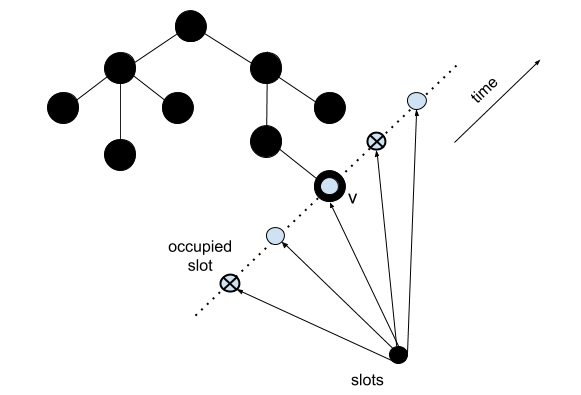
\includegraphics[width=0.7\textwidth]{spacial_temporal.png} \end{center}
\caption{Event space presented for node $v$. Nodes whose color is black form the
tree from the tree caching problem.  We add new dimension - time. Every node is
replaced by slots $(v, t)$ for discrete values of $t$, which are rounds numbers.
On the picture the new dimension is presented only for $v$.}
\label{fig:spacial_temporal} \end{figure}

As we now know, what the event space and slots are, we can define $fields$.
Fields form disjoint partition of phase $P$ (partition of slots corresponding to
$P$). Formally, if $X_t$ is changeset applied by \textbf{TRC} at time $t$, we
define related field as: $$F^t = \{(v, t'): v \in X^t \wedge last_v^t < t' \leq
t\},$$ where $last_v^{t'}$ stands for the last time strictly before $t'$ in
phase $P$, when node $v$ changed its state in the cache either by being fetched
or evicted. If there was no such change for $v$ in phase $P$ before $t'$, we
assign $last_v^{t'} = \mathrm{begin_P}$. $F^t$ is \textit{positive} if the
corresponding changeset $X_t$ is positive, similar for the \textit{negative}
field. We define $req(F^t)$ to be the occupied slots from $F^t$. Notice that
$req(F^t)$ are exactly the requests that 'paid' for changeset $X_t$, so it could
have been applied. With Lemma \ref{thm:lemma1}, we can summarize discussion
above in a simple observation.  \begin{observe} For field $F^t$ we have
$req(F^t) = |X_t| \cdot \alpha$ and the requests in one field are either all
positive or all negative.  \label{obs:observe1} \end{observe} The rest of the
event space (occupied slots that does not belong to any field $F^t$ of the phase
$P$), we call \textit{the open field} and denote by $F^{\infty}$. All fields
except of the open field are denoted by $\mathcal{F}$ and their overall size by
$|\mathcal{F}| = \sum_{F^t \in \mathcal{F}} |X^t| \cdot \alpha$.  Additionally,
for any field $F$, if $A$ is a set of nodes, $F \cap A = \{(v,t) \in F: v \in
A\}$ and if $T$ is a set of rounds $F \cap T = \{(v, t) \in F: t \in T\}$. We
introduce another definition related to fields: $\tau$\textit{-restricted}
subfields of $F^t$, which formally are equal $$F^t_{\leq \tau} = F^t \cap \{t':
t' \leq \tau\}.$$ We can think of a $\tau$-restricted subfield as a snapshot of
field, that was taken at time $\tau$ showing which slots are occupied in $F^t$
up to the time point $\tau$.  \begin{figure} \begin{center}
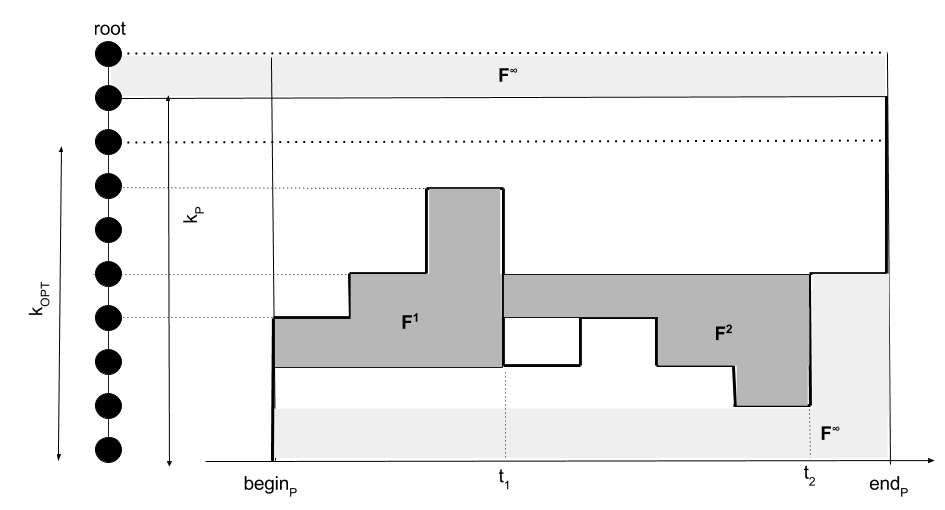
\includegraphics[width=1.1\textwidth]{fields.png} \end{center} \caption{Example
of fields for the tree structure being a line. $F^1$ is a positive field, $F^2$
is negative. $F^{\infty}$ is an open field for presented phase.}
\label{fig:fields} \end{figure} Fields are hard to visualize in general case, so
we present them only for the case when the processed tree structure forms a line
(look at the Figure \ref{fig:fields}).

Now we upper bound the cost of \textbf{TRC} obtained during phase $P$.
\begin{lemma} Let $\mathcal{F} \cup F^{\infty}$ be a partition of $P$ into
fields. We have: $$cost_{\mathrm{TRC}}(P) \leq 2 \cdot \alpha \cdot
|\mathcal{F}| + req(F^{\infty}) + k_P \cdot \alpha.$$ \label{thm:trc_cost}
\end{lemma} \begin{proof} The cost on every field $F^t$ originates from serving
requests, that belong to it and reorganizing the cache at the end of the field
(which ends with fetch or eviction). Both of this costs are equal $|X^t| \cdot
\alpha$, what substantiates the first term in right hand side of the inequality.
Expression $req(F^{\infty})$ captures all of the cost associated with the open
field in $P$ and $k_P \cdot \alpha$ is the cost of the final eviction, which
does not occur for the unfinished (last) phase. There are no other sources of
cost for \textbf{TRC}'s algorithm, so it end the proof of the lemmma.
\end{proof}

\subsubsection{Shifting} Now we proceed to the main part of our deduction. What
we need to do is to relate the cost of \textbf{OPT} with the fields. Just to
show intuition behind the idea, imagine for a moment, that requests are evenly
distributed within fields. What we mean is that each node in each field $F^t$
has exactly $\alpha$ slots occupied at the time $t$ (so we distribute $|X^t|
\cdot \alpha$ requests belonging to $F^t$ evenly). What it gives us, is that
every node $v$ alternates between time periods spent in positive and negative
field. During each such period it is requested exactly $\alpha$ times. Moreover,
we see that on two consecutive periods (first positive, then negative one)
\textbf{OPT} pays at least $\alpha$, because it changes the state of $v$ or pays
for all positive or all negative requests belonging to these two periods of $v$.
Unfortunately, we usually do not have such fair distribution of requests. What
we will do is we will change phase $P$ to $P'$, which is not harder for
\textbf{OPT} (in the sense of cost), but will take us closer to the even
distribution of the requests. It will give us then ability to lower bound the
cost of \textbf{OPT}.  \begin{figure} \begin{center}
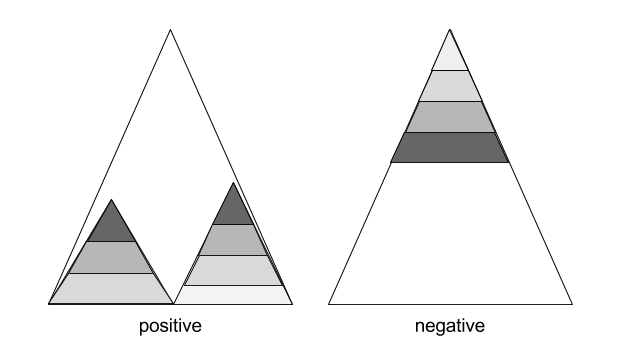
\includegraphics[width=0.8\textwidth]{density_pic.png} \end{center}
\caption{This picture shows the average density of the request in fields. The
darker the colour, the more requests are in average in that part of the
changeset.} \label{fig:density} \end{figure}

To achieve such $P'$, we will change $P$ by application of \textit{legal
shifts}.  We say, that requests placed in slot $(v, t)$ can be legally shifted
to slot $(m(v), t)$, if $v = m(v)$ or for the positive requests $m(v)$ is
descendant of $v$ or for the negative requests $m(v)$ is ascendant of $v$.
Observe, that for fixed sequence of fetches and removals from cache, for any
algorithm, the associated cost can only decrease, when the legal shifts are
applied. For example, consider positive request.  Shifting it 'down' in the tree
can lead to moving it to a node which is already in the cache and therefore we
can only save on that request. Similar example can be constructed for negative
request. We can now make the following observation: \begin{observe} If $P'$ was
created from $P$ by application of legal shifts only, then
$cost_{\mathrm{OPT}}(P') \leq cost_{\mathrm{OPT}}(P)$.  \end{observe}

We do not want changing $P$ to $P'$ to drop $cost_{\mathrm{OPT}}$ value too
much, so it would cause us being unable to argue, that it is sufficiently large.
What we want is to keep the property, that there are consecutive alternating
periods of positive and negative requests to each node, that are sufficiently
'long' in the sense of the number of requests. 

We will show that we can perform shifts within fields in such a way, that the
requests are exactly (for negative requests) or approximately (for positive
requests) evenly distributed and consequently we can lower bound \textbf{OPT}'s
cost.

Before we start presenting the way, in which we shift the requests, we
demonstrate a property of restricted subfields and their corresponding
changesets.  For any field $F$ we say that $S \subseteq F$ is
\textit{overrequested} if $req(S) > |S| \cdot \alpha$. It turns out, that some
subsets of the fields are never overrequested.  \begin{lemma} Fix $F^t$,
$F^t_{\leq \tau}$ with $X^t$ corresponding changeset.  \begin{itemize} \item If
$F^t$ is negative, then for any tree cap $T'$ of $X^t$, $T' \cap F^t_{\leq
\tau}$ is not overrequested.  \item If $F^t$ is positive, then for any
bottom-contiguous subtree $T'$ of $X^t$, $T'\cap F^t_{\leq \tau}$ is not
overrequested.  \end{itemize} \label{thm:not_over_requested} \end{lemma}
\begin{proof} We start with the proof of the property for negative fields.  From
\ref{thm:lemma1}, because $T' \cap  F^t_{\leq \tau}$ is a valid changeset at
$\tau$, we get $req(T' \cap  F^t_{\leq \tau}) = bank_{\tau}(T' \cap F^t_{\leq
\tau}) \leq |T' \cap F^t_{\leq \tau}| \cdot \alpha$. For the positive field we
have similar observation, that for any bottom-contiguous subtree $T'$ of the
positive field $T'\cap F^t_{\leq \tau}$ is a valid positive changeset, thus we
apply again \ref{thm:lemma1} obtaining desired result.  \end{proof}

Above lemma provide us a helpful attribute of the fields. Instinctively, for
positive fields the saturation of slots is more dense in average for nodes
closer to the root, whereas the density of requests in negative field is higher
at the 'bottom' (see Figure \ref{fig:density}).

For $\tau = t$ we can apply this lemma and Observation \ref{obs:observe1}, what
gives us the following corollary.  \begin{corollary} Fix $F^t$ filed with
corresponding changeset $X_t$. Let $T'$ be tree cap of $X_t$, then if the field
is: \begin{itemize} \item positive: $req(F^t \cap T') \geq |T'| \cdot \alpha$,
\item negative: $req(F^t \cap (X_t \setminus T')) \geq |X_t \setminus T'| \cdot
\alpha$.  \end{itemize} \label{thm:proper_at_t} \end{corollary}

\myparagraph{Up-shifting of negative requests}

With procedure of shifting up negative requests, we can obtain an even
distribution of requests across nodes in changeset, that corresponds to a
negative field.  \begin{theorem} By legally shifting the negative requests, we
can move requests within the negative field $F^t$ in a way, that each node has
exactly $\alpha$ requests after that procedure.  \label{thm:legal_shifting_up}
\end{theorem} To prove this theorem we will first argue, that we can always
shift requests, that appeared after first $\alpha$ requests at any leaf moving
them to the parent of that leaf. To make our argument transparent, we will say,
that a tree cap $Y \subseteq X_t$ is \textit{proper}, if for any tree cap $Y'
\subseteq Y$ and any point of time $\tau \leq t$ it holds, that $req(F^t_{\leq
\tau} \cap Y') \leq |Y'| \cdot \alpha$. Look, that Corollary
\ref{thm:proper_at_t} states, that at time $t$, being the end time of the field,
$X_t$ with all its tree caps are proper.

Now we can present a lemma, which will be then used as induction step in the
prove of Theorem \ref{thm:legal_shifting_up}.
\begin{lemma} Let $Y$ be a proper
tree cap of a negative changeset $X_t$ and let $v_l$ be one of $Y$'s leaves. If
$v_l$ was requested $r_l \geq \alpha$ times, we can legally shift  $\delta_l =
r_l - \alpha$ requests to the parent of $v_l$ (denoted $p(v_l)$), so the moved
requests are kept in $F^t$ and $Y \setminus \{v_l\}$ stays proper.
\end{lemma}
\begin{proof}
We consider $r_l$ requests, that are placed on $v_l$, in
chronological order.  See, that when $\alpha + 1$-th request comes, at time
$t_l$, $p(v_l)$ has to be in the cache. If that was not true, we would have
encountered overrequested tree cap consisting of one node $\{v_l\}$, which
contradicts Lemma \ref{thm:not_over_requested}. That means, that after $\alpha$
first requests to $v_l$, the rest $\delta_l$ requests can be moved within field
to $p(v_l)$.

What remains to be proven is that $Y' = Y \setminus \{v_l\}$, after operation
described above, is proper. Suppose it is not. Then there exists tree cap $D
\subseteq Y'$, which is overrequested at some time $\tau$. First of all $\tau
\geq t_l$, because we do not change placement of any request up to time $t_l$
and before the time $t_l$ $Y$ was proper. Also see, that $p(v)$ has to be an
element of $D$ - we did not change the number of requests in any other node.
After shift $req(F^t \cap Y) = req(F^t \cap D) + \alpha$, and if $req(F^t \cap
D) > |D| \cdot \alpha$, then $D \cup v_l$ would be overrequested, contradicting
the fact, that $Y$ is proper before change.
\end{proof}
\begin{figure}
\begin{center} 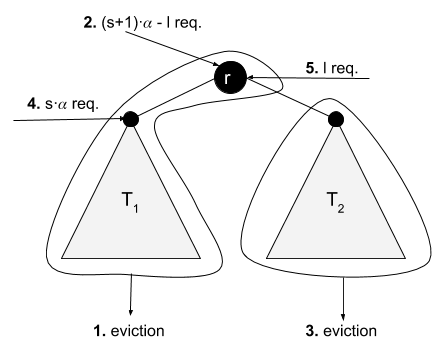
\includegraphics[width=0.8\textwidth]{example_not_even.png}
\end{center} \caption{Numbers indicate chronology of events.}
\label{fig:example_not_even} \end{figure}

Now above lemma, used as induction step, proves Theorem
\ref{thm:legal_shifting_up}. To ascertain that, recall the Corollary
\ref{thm:proper_at_t}, which ensures, that in any proper tree cap $D$ of $X_t$
there is a leaf with at least $\alpha$ requests. Going in the bottom-up manner
through the field (actually through the tree corresponding to its changeset), shifting requests from 'overrequested' nodes on the way,
leads to an even distribution of the requests - we leave $\alpha$ requests in
every node on our path. That completes the proof.

\myparagraph{Down-shifting of positive requests}

Unfortunately, we can not obtain such perfectly even distribution of requests as in the case of negative fields,
when using legal shifts on positive fields.
Specifically, we cannot shift positive requests down legally in such a way, that
we end up with $\alpha$ requests in every node. We show an example confirming
this statement. Imagine we have a tree $T$ with a root $r$ and two distinct
subtrees: $T_1$ and $T_2$, which both are of size $s$ and have $l$ leaves.
Consider the following series of events (assume, that initially whole tree $T$
is in \textbf{TRC's} cache).  \begin{enumerate} \item $T_1 \cup \{r\}$ is
evicted from cache.  \item $(s+1) \cdot \alpha - l$ requests to the root $r$
appear (no fetch occurs - there is not enough requests in $r$ to pay for whole
$T_1 \cup \{r\}$).  \item $T_2$ is evicted.  \item $s \cdot \alpha$ requests
appear at the root of $T_1$.  \item $l$ requests appear at the root $r$ of tree
$T$. $T$ is again in \textbf{TRC's} cache.  \end{enumerate}

The picture corresponding to this example can be found in the Figure
\ref{fig:example_not_even}. 
Notice, that when first $(s+1) \cdot \alpha - l$
request appear to $r$, they can only be shifted to $T_1$ nodes. After that root
of $T_1$ is given requests, which can not be moved to $T_2$. Recall, that we are
unable to do shift positive requests up. Such movement would be illegal,
therefore only $l$ last requests can be moved to $T_2$. Hence we managed to fill
only half of the tree nodes with =$\Omega(\alpha)$ requests.   

Convinced, that shifting positive request down is not so easy, our goal is to
prove, that what we can at least get by legal shifting within field $F^t$ is
$\Omega(\frac{|F^t|}{h(T)})$ nodes having $\frac{\alpha}{2}$ requests or more.
To do that first we argue, that from any node $v$ in the positive field $F^t$ we
can move down fraction of its requests, that they stay within their field and there
aren't any nodes $u$ in $T(v)$, that gets more then $\frac{\alpha}{2}$ requests
(we do not count the requests placed originally at $u$). Notice, that to shift
any request $(v, t_v)$ from $F^t$ to some node $v'$ we need to ensure, that $v'$
is outside the cache. This can be expressed by the inequality $t_v > last_{v'}(t)$.

\begin{lemma} Fix $F^t$ positive field with corresponding changeset $X_t$ and node $v \in X_t$,
that has been requested at least $c_v \cdot (\frac{\alpha}{2})$ times for some
positive integer $c_v$. There exists a legal shifting of $\lceil \frac{c_v}{2}
\rceil \cdot (\frac{\alpha}{2})$ requests, chosen from the requests to $v$, to nodes in $T(v) \cap X^t$.
Furthermore, at least $\lceil \frac{c_v}{2} \rceil$ of
these nodes are given $\frac{\alpha}{2}$ requests. All of the shifts are within
the field $F^t$.  \label{thm:request_mapping}
\end{lemma} 
\begin{proof} We sort
the elements of $T(v) \cap X_t$ with respect to the increasing time order of
element's last eviction (so with respect to function $last_v$), obtaining a sequence of nodes
$\{u_i\}_{i \geq 0}$. Since $v$ has to be in the first group of elements, that are
evicted from the cache in that field, we assume $u_0 = v$. We sort the
requests, that occurred at $v$ as well, so we get a sequence of requests sorted by the
increasing arrival time. The latter sequence will be denoted by $\{(v,
t_j)\}_{j=0}^{c_v \cdot \frac{\alpha}{2} - 1}$. We define partial function
\textit{shift} on latter sequence's elements, which will tell us to which element
among the elements of  $T(v) \cap X_t$ the argument (request) should be pushed
down. Precisely, $shift((v, t_{k \cdot \alpha + m})) = u_k$, where $m$ values are
integers taken from interval $[0, \frac{\alpha}{2})$. The function $shift$ is not
defined on the rest of the requests. We will not push those requests down. The
mapping definition given above is presented in the Figure \ref{fig:req_map}.
\begin{figure} \begin{center}
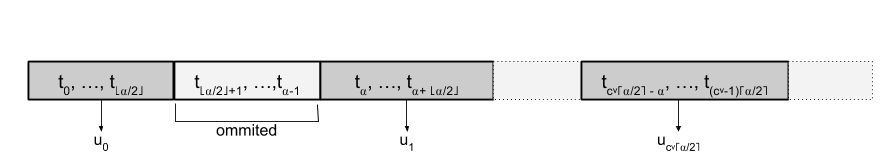
\includegraphics[width=1.1\textwidth]{request_mapping.png} \end{center}
\caption{Request mapping from Lemma \ref{thm:request_mapping}. The requests are
divided into alternating parts of size $\lceil \frac{\alpha}{2} \rceil$ and
$\lfloor \frac{\alpha}{2} \rfloor$. The odd fragments (counting from $1$) are
mapped, whereas the even parts are omitted in the mapping.} \label{fig:req_map}
\end{figure}

Now we need to prove, that defined shifting keeps requests within their fields,
so for shifted requests we need to ensure $t_j \geq last_{shift((v, t_j))}(t)$. Assume that
it is not true and $t_j < last_{shift((v, t_j))}(t)$ for a shifted request with index
$j = k \cdot \alpha + m$. Since the requests are mapped with respect to
increasing order of sequence $\{u_i\}_{i \geq 0}$, thus increasing order of $last_v$, then $|F^t_{\leq t_j} \cap T(v)| <= k$, but the
same time $|req(F^t_{\leq t_j} \cap T(v))| = j$ and $F^t_{\leq t_j} \cap T(v)$ is
then overrequested. This with Lemma \ref{thm:not_over_requested} leads to a
contradiction.
\end{proof}
We are ready to prove the main lemma of this
paragraph, which gives us possibility to obtain (nearly) even distribution of
positive request to the factor $O(\frac{1}{h(T)})$. 
\begin{lemma} For any positive field $F^t$ it is possible to shift legally $\frac{req(F^t)}{2}$
requests within the field in a way, that at least $\frac{|X^t|}{2 \cdot h(T)}$ nodes in
$F^t$ have $\frac{\alpha}{2}$ requests or more.
\label{thm:legal_shifting_down}
\end{lemma}
\begin{proof}
Let $X^t$ be corresponding changeset for $F^t$. We
take all of the requests at each node and arrange them into groups of size
$\frac{\alpha}{2}$ chronologically, meaning, that first $\frac{\alpha}{2}$
requests to a node are in first group and so on. If the last group is not full
(it has less then  $\frac{\alpha}{2}$ requests) then it is omitted. The number
of requests that are not omitted in set $X$ will be denoted by
$\overline{req}(X)$. Notice that  $\overline{req}(F^t) \geq |X^t| \cdot
\frac{\alpha}{2}$, since $req(F^t) = |X^t| \cdot \alpha$ and we omit at most
$\frac{\alpha}{2}$ requests at every node.  \begin{figure} \begin{center}
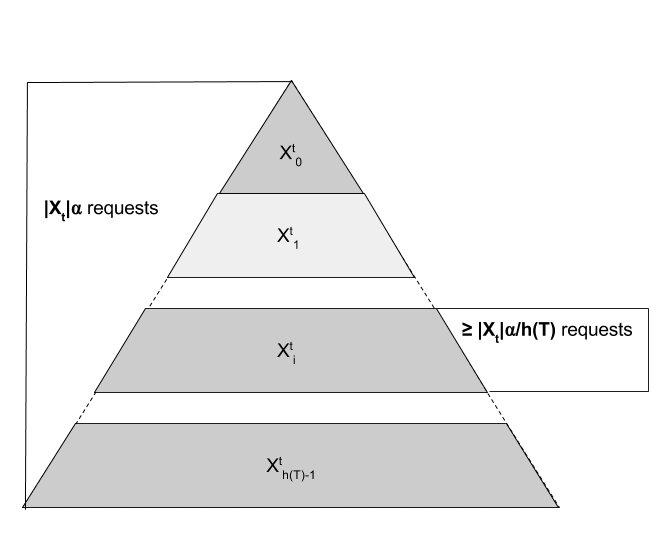
\includegraphics[width=0.5\textwidth]{layers.png} \end{center} \caption{Division
of the requests into levels. Requests to the nodes, which have the same distance
from $X^t$'s root are on the same level.} \label{fig:layers} \end{figure}

We partition the elements of $X^t$. In each part there are elements with the
same distance from the root of $X^t$. We call these parts levels. The nodes that
are at distance $i$ from the root are on level $i$ and will be denoted $X^t_i$.
We have exactly $h(T)$ levels. By pigeonhole principle, there exists a level
$X^t_i$ for which $\overline{req}(F^t \cap X^t_i) \geq \frac{req(F^t)}{2 \cdot
h(T)}$ (look at Figure \ref{fig:layers}). The subtrees, that are rooted in the nodes
of $X^t_i$ are distinct and to each of them we can apply Lemma
\ref{thm:request_mapping}. Node $v \in X^t_i$ has $\overline{req}(F^t \cap
\{v\})$ requests, so from the lemma we we can shift $\frac{\alpha}{2}$ of them
to $\lceil \overline{req}(F^t \cap \{v\}) \rceil$ distinct nodes from $T(v)$.
Summing up the 'filled' nodes for each subtree rooted in some element of
$X^t_i$, we obtain at least $\lceil \overline{req}(F^t \cap X^t_i) \rceil \geq
\frac{|X^t|}{2 \cdot h(T)}$ with at least $\frac{\alpha}{2}$ requests.
\end{proof} 
\subsubsection{Competitiveness of TRC} We will use results from
previous subsection to lower bound \textbf{OPT's} cost and finally get to the main
theorem of this thesis, which provide a bound on the competitive ratio of \textbf{TRC}
algorithm. The proofs from this subsection are mostly technical, but still
intuitions from previous sections should be useful to profoundly understand the idea
hidden behind forthcoming calculations.

We will need one auxiliary lemma about the state of \textbf{TRC's} cache at the
end of the phase. We remind, that this last cache state is somehow special - its size
exceeds $k_{\mathrm{ONL}}$, because instead of normal fetch we perform
artificial one as it was described earlier. 
\begin{lemma} 
Fix phase $P$ and the
cache state  $C$ at the end of the phase ($\mathrm{end_P}$). Any tree cap $D
\subseteq C$ received at least $|D| \cdot \alpha$ requests during the phase $P$.
\label{thm:lots_of_req_in_tc_end_of_p} 
\end{lemma}
\begin{proof}
Let $X_1, X_2,
\ldots, X_m$ be all positive changesets from the phase $P$.  We perform
separation on them, defining $X'_i = X_i \setminus \bigcup_{j=1}^{i-1} X_j$.
Note that $X'_i$ is a tree cap of $X_i$. The sequence $X'_1, X'_2, \ldots, X'_m$
is pairwise disjoint and covers $C$, so $C \subseteq \bigsqcup_{j=1}^m X'_j$.
Let $D$ be a tree cap of $C$.
Let $X_j^D = D \cap X'_j$, then $D = \bigsqcup_{j=1}^m X_j^D$, since $D
\subseteq C$. $X_j^D$ is tree cup of $X'_j$, so by transitivity of the relation
of forming a tree cap, $X_j^D$ makes up a tree cap of $X_j$. From Corollary
\ref{thm:proper_at_t} we have that $req(X_j^d \cap F_i) \geq |X_j^D| \cdot
\alpha$. There can be even more requests on the whole phase - not only
restricted to field $F_i$. Since $X_j^D$ are pairwise disjoint, we can sum up
requests over all $j$ and obtain the expected result.  \end{proof}

\myparagraph{Lower bound for OPT}

Throughout this paragraph we use a notation of $V_{\mathrm{OPT}}$. It will be
the set of nodes, that appeared in \textbf{OPT's} cache during the phase.
$V_{\mathrm{OPT}}^C$ will denote the complement to the whole tree $T$ ($T
\setminus V_{\mathrm{OPT}}$).  Notice, that $V_{\mathrm{OPT}}$ creates a proper
cache state.

We get two different lower bounds for \textbf{OPT}, which are presented in the
next two lemmas.
\begin{lemma}
For any phase $P$, $cost_{\mathrm{OPT}}(P) \geq
(k_{\mathrm{P}} - k_{\mathrm{OPT}}) \cdot \alpha$.  \label{thm:opt_bound_with_k}
\end{lemma}
\begin{proof}
Let $C$ be the cache state of \textbf{TRC} at
$\mathrm{end_P}$ (after artificial fetch, so there is $k_{\mathrm{P}}$ elements in the
cache). We consider separately the cost of \textbf{OPT} obtained on the nodes
$V_{\mathrm{OPT}}$ and $V_{\mathrm{OPT}}^c$. For the first set, \textbf{OPT} had
to fetch at least $|V_{\mathrm{OPT}}| - k_{\mathrm{OPT}}$ nodes during the phase
paying $\alpha$ for the fetch of each element. For the second one, see that $C \setminus
V_{\mathrm{OPT}}$ is a subset of $V_{\mathrm{OPT}}^c$. Moreover, $C \setminus
V_{\mathrm{OPT}}$ is an union of disjoint tree caps of subtrees, that belong to
$C$. From Lemma \ref{thm:lots_of_req_in_tc_end_of_p} all these tree caps are
'dense', so summing up requests from them gives us at least $|C \setminus
V_{\mathrm{OPT}}| \cdot \alpha$ requests to the nodes in $C \setminus V_{OPT}$,
which belong to $V_{\mathrm{OPT}}^c$ as well, as we mentioned above. Joining
results from both cases, $cost_{\mathrm{OPT}}(P) \geq (|V_{\mathrm{OPT}}| -
k_{\mathrm{OPT}}) \cdot \alpha + |C \setminus V_{\mathrm{OPT}}| \cdot \alpha =
(|C| - k_{\mathrm{OPT}}) \cdot \alpha$, what ends the prove, since $k_P$ is
defined as the size of the cache ($|C|$) after artificial fetch.
\end{proof}
\begin{lemma}
For any phase $P$, $cost_{\mathrm{OPT}}(P) \geq
(\frac{|\mathcal{F}|}{4 \cdot h(T)} -k_P) \cdot \frac{\alpha}{2}$.
\label{thm:opt_bound_with_F} \end{lemma} \begin{proof} Let $P$ be a fixed phase.
We perform shifting on $P$, so that both Lemma \ref{thm:legal_shifting_up} and
Lemma \ref{thm:legal_shifting_down} hold. The result of this action will be
called phase $P'$. From the previous discussion it is sufficient to prove, that
$cost_{\mathrm{OPT}}(P') \geq (\frac{|\mathcal{F}|}{4 \cdot h(T)}-k_P) \cdot
\frac{\alpha}{2}$. To do so, we first focus on each node $v$ separately. See
that any node's history can be divided into alternating intervals of the time,
when it was out of the cache (and was therefore charged by receiving the
positive requests) or it was in the cache (charged by negative requests). We
call those periods $OUT$ and $IN$ respectively. The cache is empty at the
beginning of the phase, so every node's periods sequence starts with an $OUT$
period. Two consecutive $OUT$ and $IN$ periods form a \textit{stripe}. Notice,
that for each node $v$ only the last $OUT$ period in phase $P'$ might be
unpaired, thus there is at most $k_P$ unpaired periods.

Let's denote by $cnt_{\mathrm{IN}}$ and $cnt_{\mathrm{OUT}}$ the number of all
$IN$ and $OUT$ periods for all nodes in $P$  respectively. From the above
discussion, $cnt_{\mathrm{OUT}} = cnt_{\mathrm{IN}} + k_P$. The sum of all
periods (both $IN$ and $OUT$) is equal to the sum of sizes of all fields
(excluding the open field), which we already denoted by $|\mathcal{F}|$. It
implies, that $|\mathcal{F}| = cnt_{\mathrm{OUT}} + cnt_{\mathrm{IN}}$ so
$cnt_{\mathrm{OUT}} = \frac{|\mathcal{F}| + k_P}{2} \geq
\frac{|\mathcal{F}|}{2}.$

Now we will use the lemmas about shifting. From them we know that in $P'$ all
$IN$ periods consist of $\alpha$ requests and there is at least
$\frac{1}{2h(T)}$ $OUT$ periods, paired with $IN$ periods, that have at least
$\frac{\alpha}{2}$ requests. Therefore, there are at least
$(\frac{cnt_{\mathrm{OUT}}}{2h(T)} - k_P)$ stripes, whose both both have
$\frac{\alpha}{2}$ requests or more. On each such pair \textbf{OPT} pays at
least $\frac{\alpha}{2}$, because of changing nodes state in cache (thus
obtaining the cost equal to $\alpha \geq frac{\alpha}{2}$) or paying for either
positive or negative requests from that stripe.  Stripes are distinct, so the
cost of \textbf{OPT} can be bounded from below by
$(\frac{cnt_{\mathrm{OUT}}}{2h(T)} - k_P) \cdot \frac{\alpha}{2} \geq
(\frac{|\mathcal{F}|}{4h(T)} - k_P) \cdot  \frac{\alpha}{2}$.  \end{proof}

\myparagraph{Upper bound for open fields}

To prove the competitiveness of \textbf{TRC} we have to deal with the open
fields. Lemma below solves this problem.  \begin{lemma} For any phase $P$ and
its open field $F^{\infty}$, $req(F^{\infty}) \leq (k_{\mathrm{ONL}} +
k_{\mathrm{OPT}}) \cdot \alpha + 2 \cdot cost_{\mathrm{OPT}}(P)$.
\label{thm:inifinite_filed_bound} \end{lemma} \begin{proof} Let
$X_{\mathrm{end_P}}$ be the	artificially applied changeset at the time
$\mathrm{end_P}$. We divide open field $F^{\infty}$ into two disjoint sets.
First of them contains positive requests, the second: negative. Formally
\begin{gather*} F^{\infty}_{+} = \{(v, t): v \notin C_{\mathrm{end_P}} \cup
X_{\mathrm{end_P}}, t \geq last_v(\mathrm{end_P})\}, \\ F^{\infty}_{-} = \{(v,
t): v \in C_{\mathrm{end_P}}, t \geq last_v(\mathrm{end_P})\}.  \end{gather*}
Now we divide requests from $F^{\infty}$ into three distinct sets
$F^{\infty}_{-}$, $F^{\infty}_{+} \cap V_{\mathrm{OPT}}$ and $F^{\infty}_{+}
\cap V_{\mathrm{OPT}}^c$. We will bound the number of requests in each of them
separately. We can do so, since the above division forms partition, that covers
$F^{\infty}$. Therefore, $req(F^{\infty}) = req(F^{\infty}_{-}) +
req(F^{\infty}_{+} \cap V_{\mathrm{OPT}}) + req(F^{\infty}_{+} \cap
V_{\mathrm{OPT}}^c)$.

Let's start with bounding $F^{\infty}_{-}$. Since its nodes are all in the cache
state $C_{\mathrm{end_P}}$, the number of nodes in $F^{\infty}_{-}$ does not
exceed $k_{\mathrm{ONL}}$. These nodes were not evicted from the cache, which
means, that number of requests in $req(F^{\infty}_{-})$ equals at most
$k_{\mathrm{ONL}} \cdot \alpha$.

Now notice, that $req(F^{\infty}_{+} \cap V_{\mathrm{OPT}}^c) \leq
req(V_{\mathrm{OPT}}^c)$. The nodes from $V_{\mathrm{OPT}}^c$ were never in
\textbf{OPT's} cache during phase $P$, so it has to pay for all of the positive
requests to them. This gives us $req(V_{\mathrm{OPT}}^c) \leq
cost_{\mathrm{OPT}}(P)$ and finally $req(F^{\infty}_{+} \cap V_{\mathrm{OPT}}^c)
\leq cost_{\mathrm{OPT}}(P)$.

To get the bound for the ramaining set note, that $F^{\infty}_{+}$ is a valid
changeset for $C_{\mathrm{end_P}} \cup X_{\mathrm{end_P}}$. At the same time,
$V_{\mathrm{OPT}}$ forms a valid cache state. Combining these two observations,
we can conclude, that $F^{\infty}_{+} \cap V_{\mathrm{OPT}}$ is a valid
changeset for $C_{\mathrm{end_P}} \cup X_{\mathrm{end_P}}$ (and these sets'
intersection is empty). Let $X^{V}_{+}$ be the set of nodes in $F^{\infty}_{+}
\cap V_{\mathrm{OPT}}$. If $req(F^{\infty}_{+} \cap V_{\mathrm{OPT}})$ would be
greater then $|X^{V}_{+}| \cdot \alpha$, then we would have been able to extend
changeset $X_{\mathrm{end_P}}$ by these nodes, contradicting the maximality
property of changesets applied by \textbf{TRC} algorithm.  Therefore,
$req(F^{\infty}_{+} \cap V_{\mathrm{OPT}}) \leq |X^{V}_{+}| \cdot \alpha \leq
|V_{\mathrm{OPT}}| \cdot \alpha \leq k_{\mathrm{OPT}} \cdot \alpha +
(|V_{\mathrm{OPT}}| - k_{\mathrm{OPT}}) \leq k_{\mathrm{OPT}} \cdot \alpha +
cost_{\mathrm{OPT}}(P)$.

Now we can combine the inequalities discussed above and finalize the proof.
\begin{equation*} \begin{split} req(F^{\infty}) & = req(F^{\infty}_{-}) +
req(F^{\infty}_{+} \cap V_{\mathrm{OPT}}) + req(F^{\infty}_{+} \cap
V_{\mathrm{OPT}}^c) \\ & \leq (k_{\mathrm{ONL}} \cdot \alpha) +
(k_{\mathrm{OPT}} \cdot \alpha + cost_{\mathrm{OPT}}(P)) +
(cost_{\mathrm{OPT}}(P)) \\ & = (k_{\mathrm{ONL}} + k_{\mathrm{OPT}}) \cdot
\alpha + 2 \cdot cost_{\mathrm{OPT}}(P) \end{split} \end{equation*} \end{proof}
\myparagraph{Main result}

Now we are ready to state and prove the main result.  \begin{theorem} Algorithm
\textbf{TRC} is $O(\frac{h(T) \cdot k_{\mathrm{ONL}}}{k_{\mathrm{ONL}} -
k_{\mathrm{OPT}} + 1})$-competitive.  \label{thm:main_theorem} \end{theorem}
\begin{proof} It is sufficient to show, that for any phase $P$,
$\frac{cost_{\mathrm{TRC}}}{cost_{\mathrm{ONL}}} = O(\frac{h(T) \cdot
k_{\mathrm{ONL}}}{k_{\mathrm{ONL}} - k_{\mathrm{OPT}} + 1})$. Then summing up
the cost over all the phases will give us the desired result.

We fix phase $P$. Recall, that from Lemma \ref{thm:trc_cost} we know, that
$cost_{\mathrm{TRC}}(P)$ is bounded by sum $2 \cdot \alpha \cdot |\mathcal{F}| +
req(F^{\infty}) + k_P \cdot \alpha$. We bound the first two summands using the
inequalities from lemmas, that we stated in previous sections. Firstly, from
Lemma \ref{thm:opt_bound_with_F} we can derive, that $|\mathcal{F}| \leq 4h(T)
\cdot (cost_{\mathrm{OPT}}(P) + k_P \cdot \alpha)$. Secondly, from Lemma
\ref{thm:inifinite_filed_bound} we have $req(F^{\infty}) \leq (k_{\mathrm{ONL}}
+ k_{\mathrm{OPT}}) \cdot \alpha + 2 \cdot cost_{\mathrm{OPT}}(P) \leq 2 \cdot
(k_P \cdot \alpha + cost_{\mathrm{OPT}}(P))$. Therefore, $2 \cdot \alpha \cdot
|\mathcal{F}| + req(F^{\infty}) = O(h(T)) \cdot (k_P \cdot \alpha +
cost_{\mathrm{OPT}}(P))$.  \end{proof}

\subsection{Lower bound for competitive ratio} We will now show, that the
competitive ratio, which is the result of the Theorem \ref{thm:main_theorem} is
optimal up to factor $O(h(T))$. We prove this statement by justifying, that any
online algorithm has to be at least $\Omega
(\frac{k_{\mathrm{ONL}}}{k_{\mathrm{ONL}}- k_{\mathrm{OPT}} + 1})$.
\begin{theorem} For any value $\alpha$ being a cost of changing one element's
state in the cache, any online algorithm for the tree caching problem is at
least $\Omega (\frac{k_{\mathrm{ONL}}}{k_{\mathrm{ONL}}- k_{\mathrm{OPT}} +
1})$-competitive.  \end{theorem} \begin{proof} To prove this theorem we will use
the Theorem 5 from publication \cite{tarjan}. The result from this article
states that any online algorithm solving the standard paging problem (move from
slow memory to fast memory costs $1$ and there is no bypassing) is at least
$\Omega(\frac{k_{\mathrm{ONL}}}{k_{\mathrm{ONL}}- k_{\mathrm{OPT}} +
1})$-competitive. What is sufficient to do is to construct a bijective mapping
from any online algorithm for paging problem to an online algorithm forthe tree
caching problem and mapping from any input for the paging problem to an input
for the tree caching problem. We can loose only constant factor on the cost,
when performing both algorithms on the corresponding inputs.

We equate all pages $p$ from the paging problem fixing a bijection $f$ from the
pages to leaves $l \in T$, so $f(p) = l$. Let's define the mapping between
inputs. By $I$ denote the input for the paging and by $I'$: input for the tree
caching problem. We change $I$ sequence, going through its requests one by one.
Whenever there is request to $p$, we add to $I'$ exactly $\alpha$ requests to
$f(p)$. Now we would like to argue that, for any online algorithm for the paging
problem $A$, that pays $c$ on input $I$, we can construct algorithm $A'$ for the
tree caching problem, that on input $I'$ pays $\theta(c \cdot \alpha)$. We
define $A'$ as follows.  When $A$ serves request $r$ from $I$ and fetches $r$ to
its cache, algorithm $A'$ bypasses corresponding $\alpha$ requests to $f(r)$ and
fetches $r$. If $A$ evicts some pages, $A'$ evicts leaves corresponding to that
pages. Notice, that $A'$ has the same cache state as $A$, as long as we apply
$f$ on its elements and look at its state every $\alpha$ (for $A$ - every one)
requests. Therefore, if $A$ does not pay for some request, then $A'$ does not
pay for it neither. $A'$ pays then at most $O(\alpha)$ times more then $A$ (all
eviction operations' cost on the sequence $I'$ has asymptotically the same value
as all fetch operations' cost).

We can inverse the reduction above and see that $A$ pays on $I$ is
$O(\frac{1}{\alpha})$ times the cost of $A'$.    \end{proof}
